\documentclass{article}
\usepackage[utf8]{inputenc}
\usepackage{graphicx}
\title{Actividad 5}
\author{Roberto Alexis Gomez Pintor}
\begin{document}
\maketitle
\section{Introduccion}
En esta actividad haremos uso del editor Emacs para prepar los datos obtenidos de la actividad 4, luego usandolos en Panda. Como sabemos ya tenemos obtuvimos 12 archivos de datos referente a cada mes del año 2017 en la estacion 34467 en Vologrado, Rusia, con esos datos usaremos los comandos grep y wc para modificar, el archivo sondeos.txt que fue la union de los 12 archivos originales.
\section{Descripción de los conceptos físicos de CAPE y PW, que se obtienen de los datos de sondeos de la parte alta de la atmósfera.}
\subsection{CAPE}
En meteorología, la energía potencial convectiva disponible (CAPE), es la cantidad de energía que tendría una parcela de aire si se levantara una cierta distancia verticalmente a través de la atmósfera. CAPE es efectivamente la flotabilidad positiva de un paquete de aire y es un indicador de la inestabilidad atmosférica, lo que lo hace muy valioso para predecir el mal tiempo. 
\subsection{PW}
El agua precipitable es la profundidad del agua en una columna de la atmósfera, si toda el agua en esa columna se precipitó como lluvia. Como profundidad, el agua precipitable se mide en milímetros o pulgadas. A menudo abreviado como "TPW" = agua precipitable total.
\section{Descripción del proceso de limpieza y preparación de los datos para posteriormente analizar con Pandas.}
El proceso de inicio tomando el archivo df2017 que es el resultando del sondeos.txt obtenido en la actividad 4, vemos que teniendo varios datos que no se utilizaran, haciendo que solo debemos dejar el CAPE y PW como unicos datos importantes contando las fechas que se registraron. Usando el editor de textos Emacs y los comandos necesarios, logramos obtener el archivo que se utilizara para trabajar.
\section{Análisis de datos utilizando Pandas.}
Los datos analizados vemos que dejo un archivo con 2 horas, una de ellas corresponde a las 00(12:00 am) y otra las 12(12:00 pm) aqui hacemos que se divida en 2 archivos, uno decidado a las horas 00 y otro a las horas 12. Dejando con los datos PW y CAPE.
\section{Resultados del analisis}
El analisis dio como resultado las graficas referentes de CAPE y PW contra el tiempo medido en meses y entre si mismas.
\begin{figure}
  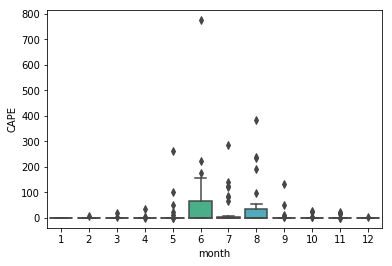
\includegraphics[width=\linewidth]{mescape.png}
  \caption{Grafica de CAPE contra tiempo.}
\end{figure}
\begin{figure}
  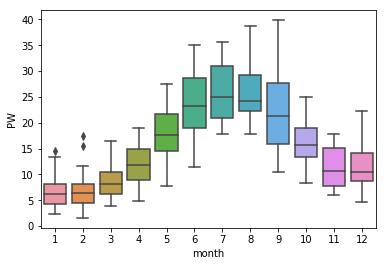
\includegraphics[width=\linewidth]{mespw.png}
  \caption{Grafica de PW contra tiempo}
\end{figure}
\begin{figure}
  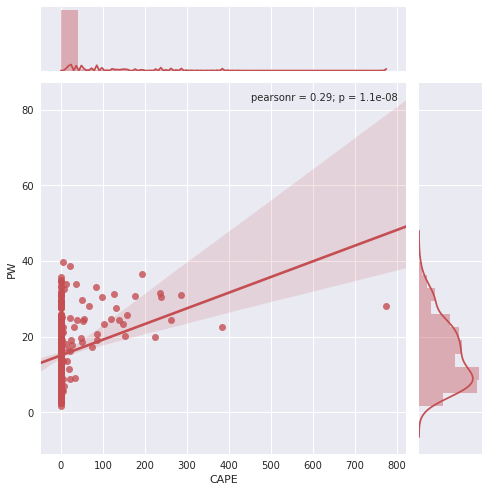
\includegraphics[width=\linewidth]{capepw.png}
\end{figure}
\begin{figure}
  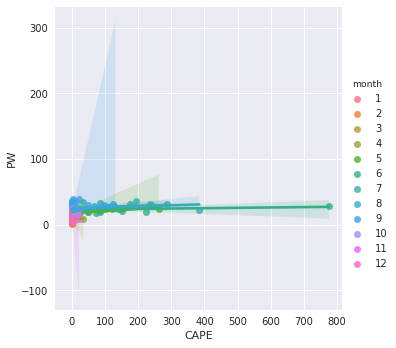
\includegraphics[width=\linewidth]{capepwcolor.png}
\end{figure}
\section{Conclusiones}
Podemos observar que tanto el CAPE como PW tienen relacion con el tiempo debido a que ahi un aumento en la PW en los meses de junio a semptiembre. 
\subsection{Preguntas}
\subsubsection{¿Cómo se te hizo esta actividad? ¿Compleja, Difícil, Sencilla?}
Algo compleja por el uso constante de los comandos de emacs, pero una vez con la ayuda indicada pude seguir avanzando a terminar el trabajo.
\subsubsection{¿Qué te llamó más la atención?}
El parecido con la actividad anterior al modificar todavia mas la informacion obtenida de los sondeos.
\subsubsection{¿Qué parte fue la que menos te interesó hacer?}
EL uso de pandas en Juypyter Notebook, debido a que un error mio en el archivod e trabajo tenia un espacio, provocando que me detuviera para ver que error pasaba.
\subsubsection{¿Cómo mejorarías esta actividad? ¿Qué le faltó? ¿Qué sobró?}
No encuentro algo que mejorar.
\subsubsection{¿Hasta este punto, que te parece el uso de Jupyter para programar en Python?}
Pues parece buen uso al usarlo, aunque complica con la construccion del codigo para usarlo, pero a patir de eso no ahi mucha complicaciones.

\end{document}
